
\chapter{Convolutional Neural Networks}

\section{Introduction}

\subsection{Idea} In order to introduce convolutional neural networks, let's explore the role they play in neural networks.
A neural network architecture should be chosen in accordance to the type of structure of input data. Consider the following example.

\begin{example}
A data matrix X containing data such as statistics on houses with no real structure may use a fully connected architecture. Instead, let's take the example where X is a matrix with rows  of image pixel data. \\\\ Take this image to be a black and white image thay may be represented by a 3x3 matrix of pixels where each pixel is a level of "darkness" defined by the values: 0,1,2,3.\\

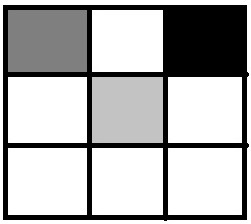
\includegraphics[scale=0.40]{images/Chapter 11/pic1.png}
\quad
\\
Pixels may be placed in a row by arranging the columns in order of their index as features.\\\\
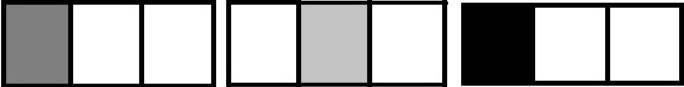
\includegraphics[scale=0.40]{images/Chapter 11/pic2.png}
\\\\
We get the vector $(x_1,x_2,x_3,x_4,x_5,x_6,x_7,x_8,x_9)$.
Note that in the 3x3 matrix, $x_4$ is near $x_1$ and $x_7$, but the vector looses this structure. \\\\
This is our motivation for introducing a new type of layer to our neural network called a convolutional layer, in order to preserve a particular "structure" of the image. 

\end{example}


\section{Convolutional Layers}
\subsection{Convolutional Layer with 1D Inputs}
%---------------definition----------------------------------------------------------
\begin{definition}
%undefined control sequence?
    A discrete 1-D signal is a sequence $y=(y_i)_{i\in\mathbb{Z}}$ of real numbers and is $L^1$-finite if $\sum |y_k| < \infty$ and compact if there exists N such that $|k| > N$ implies $y_k=0$.
    A 1-D kernel is a compact support signal of weights, w. Where $w = (w_i)_{i\in\mathbb{Z}}$. Since usually we want w to be a probability distribution, then $\Sigma_{i}w_i = 1$.
\end{definition}
%----------------------------------------------------------------------------------
%undefined control sequence?
Thus, the convolution, often called the cross correlation in signal processing, of y and w is $z=y*w$ where $z_{j} = \sum_{k\in\mathbb{Z}} y_{y+k}w_{k}$
%---------------example 2----------------------------------------------------------
\begin{example} \quad
\\
let
$w_i = \begin{cases}
    1/2 &\text{if} \quad i=0,1\\
    0 &\text{else}
\end{cases}$
\\
So $(y+w)_i=\sum_{k\in\mathbb{Z}} y_{i+k}w_k=\frac{y_i+y_{i+1}}{2}$
\end{example}
%-----------------------------------------------------------------------------------
\noindent
\\
More generally,
$w_i = \begin{cases}
    1/M &\text{if} \quad i=0,...,M-1\\
    0 &\text{else}
\end{cases}$
\\
%undefined control sequence?
Now $(y+w)_i=\sum_{k\in\mathbb{Z}} y_{i+k}w_k=\frac{y_i+y_{i+1}+...+y_{i+M-1}}{M}$
\\
\begin{example} \quad
\\
let $y=(1,2,3,4,5,6)$ and $w=(\frac{1}{2},\frac{1}{2})$
\\
Here $y+w = (\frac{1}{2},\frac{3}{2},\frac{5}{2},\frac{7}{2},\frac{9}{2},\frac{11}{2},3)=\frac{y_i+y_{i+1}}{2}$
\\
The operation is as follows
\\\\
$\begin{pmatrix}
\frac{1}{2}&\frac{1}{2} & & & & & &\\
& \frac{1}{2}&\frac{1}{2} & & & \text{\huge0}& &\\
&& \frac{1}{2}&\frac{1}{2} & & & &\\
&&& \frac{1}{2}& \frac{1}{2} & & &\\
&&&&\frac{1}{2} &\frac{1}{2} & &\\
&&\text{\huge0}&&&\frac{1}{2} &\frac{1}{2} &\\
&&&&&&\frac{1}{2} &\frac{1}{2}
\end{pmatrix}$
$\begin{pmatrix}
1\\2\\3\\4\\5\\6
\end{pmatrix}$
=
$\begin{pmatrix}

\frac{1}{2}(0) + \frac{1}{2}(1)\\
\frac{1}{2}(1) + \frac{1}{2}(2)\\
\frac{1}{2}(2) + \frac{1}{2}(3)\\
\frac{1}{2}(3) + \frac{1}{2}(4)\\
\frac{1}{2}(4) + \frac{1}{2}(5)\\
\frac{1}{2}(5) + \frac{1}{2}(6)\\
\frac{1}{2}(6) + \frac{1}{2}(7)\\
\end{pmatrix}
$
=
$
\begin{pmatrix}
\frac{1}{2}\\
\frac{3}{2}\\
\frac{5}{2}\\
\frac{7}{2}\\
\frac{9}{2}\\
\frac{11}{2}\\
3\\
\end{pmatrix}
$
\end{example}
\quad
\\
\noindent
When we use this in a neural network layer, we usually ignore the first and last component. We may also ignore some parts on the inside or only use alternating entries.

\subsection{Convolutional Layer with 3D Inputs}
\begin{example}\label{ex:CNNanimal}
In this example, we look at a neural network which uses two convolutional layers that takes images of animals and outputs a prediction of cat, dog, bear or pig.

\begin{figure}[H]
    \centering
    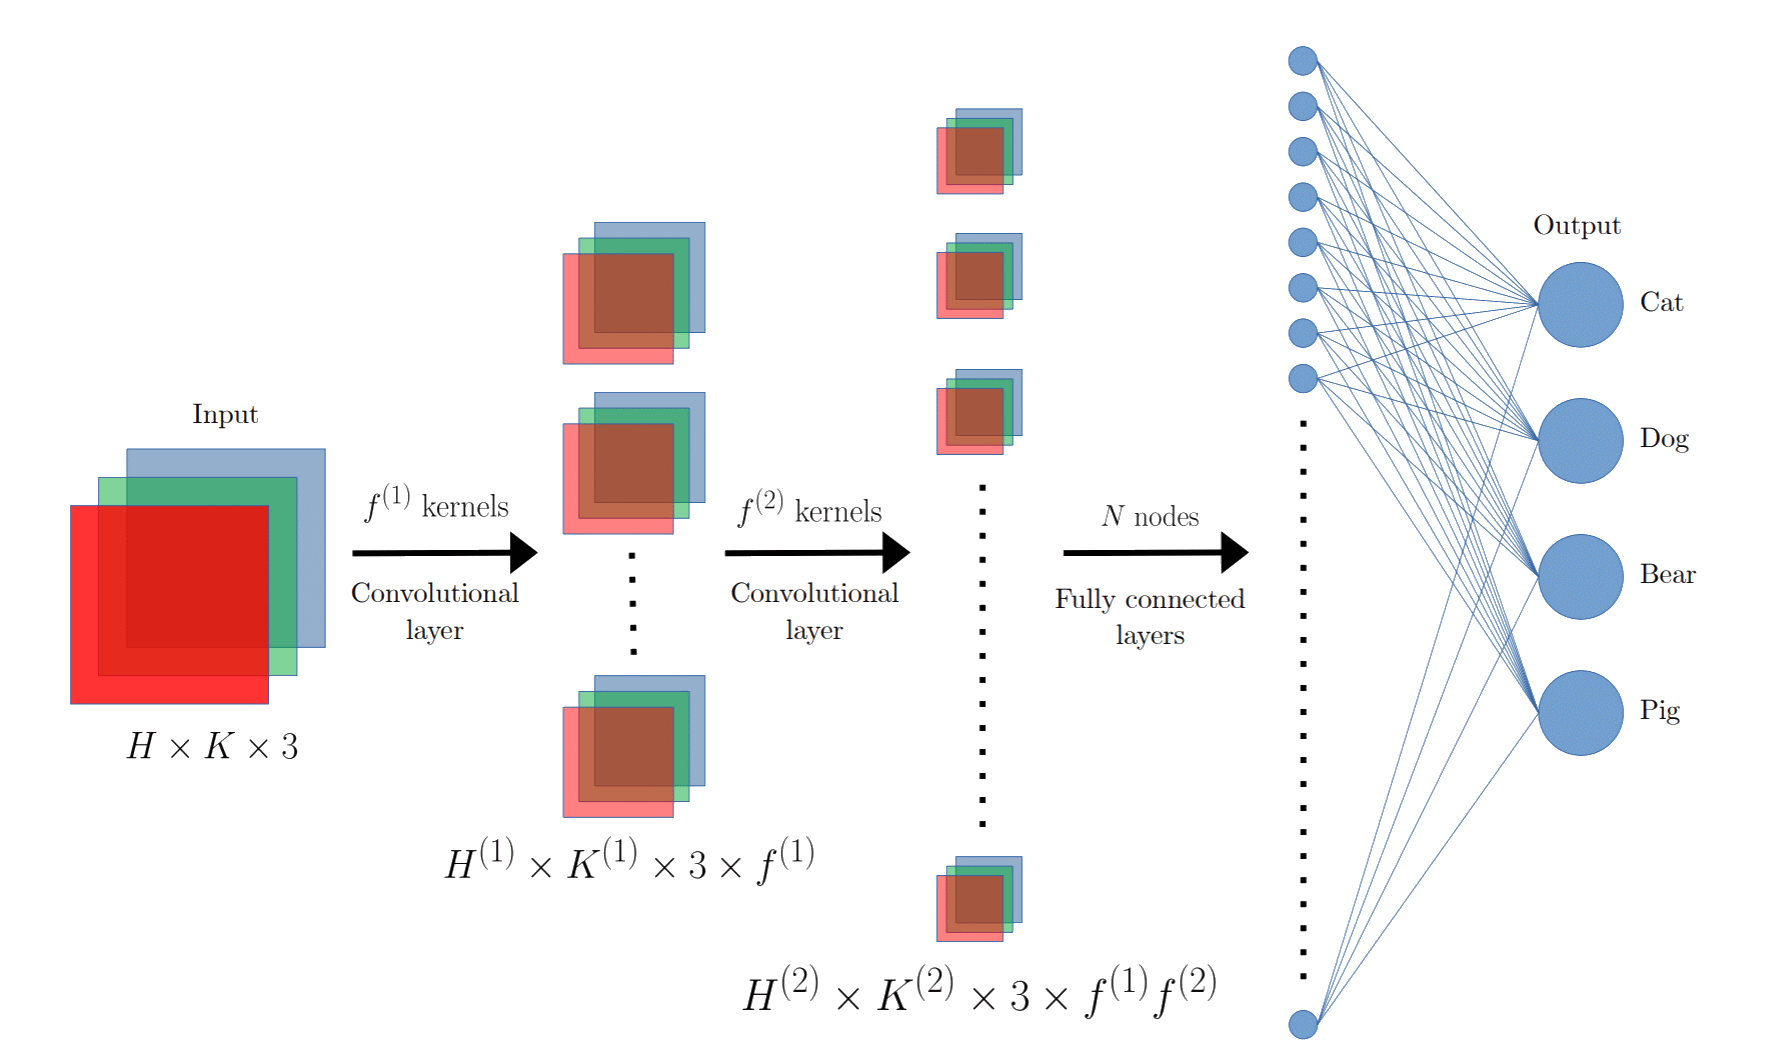
\includegraphics[scale=0.35]{images/Chapter 11/convolutionalNNexample.png}
    \caption{Neural network using convolutional layers to predict images of cat, dog, bear and pig.}
    \label{fig:11.1}
\end{figure}
The input consists of images of animals stored as $H\times K$ dimensions with $3$ color channels containing its associated RGB data. As discussed in the previous section, every signal passing through a convolutional layer will increase the number of features multiplicatively. This can be see in the formula to compute the $l$-th signal $Z^{(l)}$ given kernel $W^{(l)}$, bias $b^{(l)}$ and previous signal $Z^{(l-1)}$ which has $f_in$ features:
$$Z_{i,j,c,(f_{\text{in}},f_{\text{out}})}^{(l)} = G \left[ \left( \sum_{s,p}Z^{(l)}_{i+p,j+s,c,f_{\text{in}}} W_{p,s,c,(f_{\text{in}},f_{\text{out}})}^{(l)} \right) + b^{(l)}_{i,j,c,(f_{\text{in}},f_{\text{out}})}\right].$$

\noindent In this case, and in general, we find that
\begin{ceqn}
    \begin{align*}
        H^{(2)} &\leq H^{(1)} \leq H\\
        K^{(2)} &\leq K^{(1)} \leq K\\
        f^{(1)}f^{(2)} &\geq f^{(1)} \geq 1
    \end{align*}
\end{ceqn}
$H^{(l)}$ and $K^{(l)}$ is nonincreasing since we are applying convolution (see [relevant section when it gets written]). Sometimes, we want to preserve the size of $H^{(l)}$ and $K^{(l)}$ in all layers of our network. Moreover, the number of nodes $N$ in the example can be very large and computationally costly. To mitigate this problem, we introduce a padding and pooling process into our neural network.\\
\end{example}
\subsection{Padding}
\begin{definition}\label{def:Def11.1.1}
    For any matrix $\textbf{A} \in \mathbb{R}^{m,n}$, a \define{$p-$padding} applied to $\textbf{A}$ is the transformation $\textbf{I}_L\textbf{A}\textbf{I}_R$, where $\textbf{I}_L \in \mathbb{R}^{m+2p\times m}$ and $\textbf{I}_R \in \mathbb{R}^{n \times n+2p}$ such that
    $$(\textbf{I}_L)_{i,j} = \begin{cases} 1 & \text{ if } i = j-1 \text{ and } p+1 \leq i \leq m + 2p - 1\\ 
    0 & \text{ else } \end{cases}$$
    and
    $$(\textbf{I}_R)_{i,j} = \begin{cases} 1 & \text{ if } j = i+1 \text{ and }  p+1\leq j \leq n+2p-1\\ 
    0 & \text{ else } \end{cases}$$
\end{definition}
In simpler terms, if we have a matrix $\textbf{A} = \begin{bmatrix} a_{1,2} & a_{2,2} \\ a_{2,1} & a_{2,2} \end{bmatrix}$ and we apply $1-$padding to this, we will obtain a result of the form
$$\textbf{A}_{\text{padded}} =
\begin{bmatrix}
0 & 0 & 0 & 0 \\
0 & a_{1,1} & a_{1,2} & 0 \\
0 & a_{2,1} & a_{2,2} & 0 \\
0 & 0 & 0 & 0
\end{bmatrix}
$$
That is, we ``surround" the entries of $\textbf{A}$ with zeros.\\

\noindent Now suppose we have a $4 \times 4$ image, and we perform a convolution with stride $1$ and kernel of size $(2 \times 2)$. Then
$$
(4 \times 4) \ast_{(1,1)} (2 \times 2) = (3 \times 3)
$$
% To apply a 1-padding, we ``surround" our $(4 \times 4)$ input matrix with zeros, i.e.

% \begin{ceqn}
%     \begin{align*}
%     H = 
%         \begin{bmatrix}
%             0 & 0 & 0 & 0 & 0 & 0 \\
%             0 & H_{1,1} & H_{1,2} & H_{1,3} & H_{1,4} & 0\\
%             0 & H_{2,1} & H_{2,2} & H_{2,3} & H_{2,4} & 0\\
%             0 & H_{3,1} & H_{3,2} & H_{3,3} & H_{3,4} & 0\\
%             0 & H_{4,1} & H_{4,2} & H_{4,3} & H_{4,4} & 0\\
%             0 & 0 & 0 & 0 & 0 & 0 
%         \end{bmatrix}
%         %     \ast_{(1,1)}
%         % \begin{bmatrix}
%         % W_{1,1} & W_{1,2} \\
%         % W_{2,1} & W_{2,2}
%         % \end{bmatrix}
%     \end{align*}
% \end{ceqn}

\noindent Then by applying convolution to this with kernel of size $(2 \times 2)$, the result is of size $(5 \times 5)$. Unfortunately, the size is not preserved, and we instead get an increase in the image size. However, there is a $p$ value to pad which preserves the size faithfully, and we investigate the general case for a square filter. \\

\begin{proposition}
For a matrix $\textbf{A} \in \mathbb{R}^{H \times K}$ and kernel $\textbf{W} \in \mathbb{R}^{h \times k}$, if $h = k$ and $h$ is odd, then a $p-$padding with $p = \frac{h-1}{2}$ applied to $\textbf{A}$ preserves its size after convoluting with $\textbf{W}$.
\end{proposition}
\begin{proof}
Since the size of $\textbf{A}$ after convoluting with $\textbf{W}$ is $(H+2p)-h+1 \times (K+2p)-h+1$, solving $H+2p-h+1 = H$ yields $p = \frac{h-1}{2}$. The restriction that $h$ is odd ensures that $p$ is an integer.
\end{proof}

\begin{definition}
    A padding which preserves size is called ``same" padding.
\end{definition}

\subsection{Pooling}
When dealing with very large matrices, it is often useful to reduce their size to achieve better computational efficiency whilst preserving pertinent data of the original matrix. In neural networks which receive matrices of variable data sizes, pooling can also be used to compress them into similar sizes to compute. This is the motivation behind pooling.

\begin{definition}
    A \define{local pooling} consists of partitioning (in some way) $\textbf{A}^{m \times n}$ and computing a local statistic (e.g. maximum, minimum or average).
\end{definition}

\begin{example}
    Given matrix
    $$\textbf{A} = 
    \begin{bmatrix}
        1& 2& 3 &1\\
        1 &5&2 &7 \\
        10& 1& 2& 4\\
        8& 9& 1 &8
    \end{bmatrix},
    $$we pool $\textbf{A}$ by partitioning it into four squares of size $2 \times 2$ each (that is, $A_{1} = \{1,2, 1,5 \}$, $A_{2} = \{ 3,1,2,7\}$, $A_{3} = \{ 10,1,8,9\}$, $A_{4} = \{ 2,4,1,8\}$) and computing the maximum of each partition and store the result into a $2 \times 2$ matrix:
    \begin{ceqn}
        \begin{align*}
            \textbf{A}_{\text{pool}} &= \begin{bmatrix} \max\{ i : i \in A_{1}\} & \max\{ i : i \in A_{2}\} \\
            \max\{ i : i \in A_{3}\} & \max\{ i : i \in A_{4}\}
            \end{bmatrix}\\
            & =
            \begin{bmatrix}
                5 & 7 \\
                10 & 8
            \end{bmatrix}
        \end{align*}
    \end{ceqn}
\end{example}

\begin{definition}
    A \define{global pooling} is a local pooling between two or more matrices.
\end{definition}
\begin{example}
    Global pooling is highly useful in reducing the rank of a tensor. In \textbf{Example} \ref{ex:CNNanimal}, given the 4-tensor signal $Z^{(l)}_{i,j,c,(f_{\text{in}},f_{\text{out}})}$, globally pooling over $i,j$ with respect to maximum yields $Z'^{(l)}_{c,(f_{\text{in}},f_{\text{out}})}$ which is a 2-tensor.
\end{example}

\begin{example}
To illustrate the power of pooling in terms of computational efficiency, we return to the neural network given in \textbf{Example} \ref{ex:CNNanimal}, and introduce pooling to reduce the size of our image at each step.
  \begin{figure}[H]
    \centering
    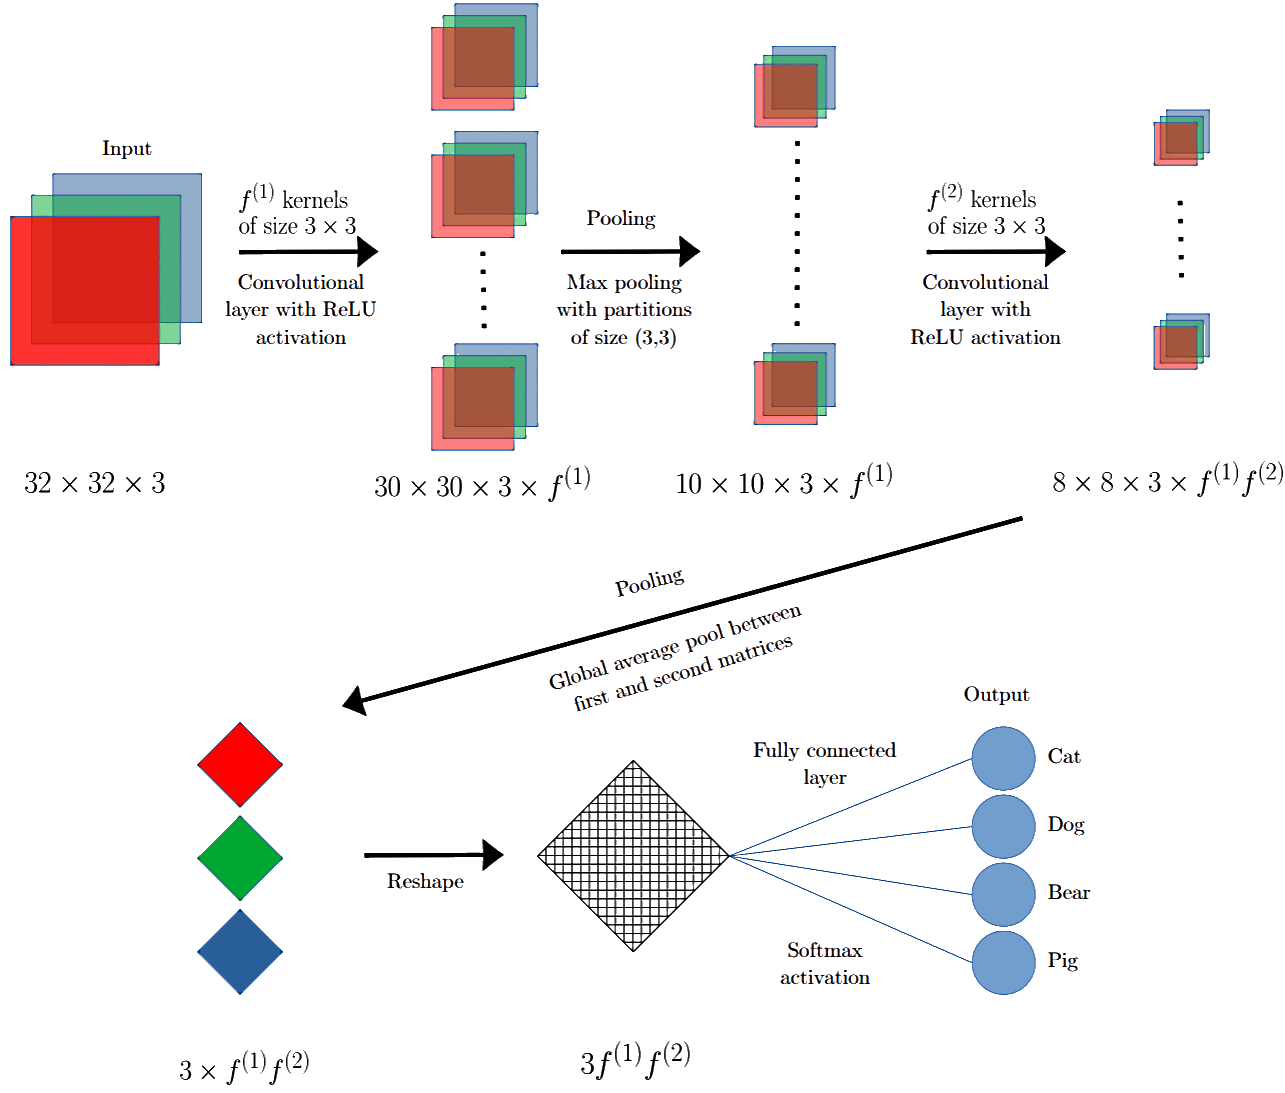
\includegraphics[scale=0.35]{images/Chapter 11/poolingNetwork.png}
    \caption{Neural network using convolutional layers and pooling to predict images of cat, dog, bear and pig. Note that the image size decreases at each step.}
    \label{fig:11.1}
\end{figure}
\noindent Now the fully connected layer at the last step involves only a single scalar output of magnitude $3f^{(1)}f^{(2)}$, instead of flattening a $H^{(2)} \times K^{(2)} \times 3 \times f^{(1)}f^{(2)}$ in the original architecture. It is good practice is to pool the data after each convolutional operation, as consecutive convolutional operations are computationally costly.
\end{example}

\section{Exercises}
\begin{enumerate}
    \item For matrices $\textbf{X}_1, \ldots, \textbf{X}_n$ with entries in $\mathbb{R}$ and size $m_{\textbf{X}_j}$ and $n_{\textbf{X}_j}$ respectively of $\textbf{X}_j$, define $\max\{{\textbf{X}_1,\ldots,\textbf{X}_n}\} = \max\{{i : i \in \textbf{X}_1 \vee \ldots \vee i \in \textbf{X}_n}\}$, $\min\{{\textbf{X}_1,\ldots,\textbf{X}_n}\} = \min\{{i : i \in \textbf{X}_1 \vee \ldots \vee i \in \textbf{X}_n}\}$ and $\text{avg}\{{\textbf{X}_1,\ldots,\textbf{X}_n}\} = \frac{1}{n}\sum_{s,t}(\textbf{X}_j)_{s,t}$.\\
    
    Compute the global pool of $\textbf{A},\textbf{B}$ and $\textbf{C}$ below, storing your result in $\textbf{v} \in \mathbb{R}^3$ where $\textbf{v} = ( \max\{\textbf{A},\textbf{B},\textbf{C} \}, \min\{\textbf{A},\textbf{B},\textbf{C} \},\text{avg}\{\textbf{A},\textbf{B},\textbf{C} \} )$.
        $$\textbf{A} = \begin{bmatrix}
                1 & 2 \\
                -3 & 4
            \end{bmatrix},\;\textbf{B} = \begin{bmatrix}
                13 & -2 \\
                6 & 1
            \end{bmatrix},\;\textbf{C} = \begin{bmatrix}
                1 & 2 \\
                7 & 5
            \end{bmatrix}$$
            
    \item Given $\textbf{I}_L$ and $\textbf{I}_R$ defined in \textbf{Definition }\ref{def:Def11.1.1}, explicitly write down the entries of $\textbf{I}_L$ and $\textbf{I}_R$ for the $1-$padding of 
    $$\textbf{A} = \begin{bmatrix}
        5 & 3 \\
        8 & 2
    \end{bmatrix}.$$
    
    \item Write an algorithm or a pseudocode which computes the $p-$padding of a matrix. The inputs should consist of the matrix itself and $p$, and output should consist of the padded matrix.
\end{enumerate}

\section{Solutions to Exercises}
\begin{enumerate}
    \item $\textbf{v} = (13,-3,\frac{37}{3})$
            
    \item $$\textbf{I}_L = \begin{bmatrix}
        0 & 0 \\ 1 & 0 \\ 0 & 1 \\ 0 & 0
    \end{bmatrix}, \textbf{I}_R = \textbf{I}_L^{\top}$$
    
    \item Inputs are matrices $\textbf{X}$, and a natural number $p$. We will use Python-like pseudocode and Numpy methods, although their operations can be generalized to any language which support such features.
    \begin{algorithm}
    \caption{$p-$padding(\textbf{X},$p$)}
    \begin{algorithmic}[1]
        \State $m,n$ = \text{\textbf{X}.shape[0], \textbf{X}.shape[1]}
        \State $\textbf{I}_L, \textbf{I}_R$ = \text{np.eye(m)},\;\text{np.eye(n)}
        \State rowZero = np.atleast\_2d(np.zeros($\textbf{I}_L$.shape[1]))
        \State colZero = np.atleast\_2d(np.zeros($\textbf{I}_R$.shape[1]))
        \State colZero = colZero.$\top$
        \State $\textbf{I}_L$ = np.concatenate(($\textbf{I}_L$,rowZero), axis=0)
        \State $\textbf{I}_L$ = np.concatenate((rowZero,$\textbf{I}_L$), axis=0)
        \State $\textbf{I}_R$ = np.concatenate(($\textbf{I}_R$,colZero), axis=1)
        \State $\textbf{I}_R$ = np.concatenate((colZero,$\textbf{I}_R$), axis=1)
		\If {$p > 1$}
		\State \Return $p-$padding($\textbf{I}_L\textbf{X}\textbf{I}_R, p-1$)
		\EndIf
        \State \Return $\textbf{I}_L\textbf{X}\textbf{I}_R$
	\end{algorithmic} 
\end{algorithm}
\end{enumerate}








